\newpage
\section{Ausgangssituation}
\subsection{IST-Analyse}
\subsubsection{Unternehmensvorstellung}
Das Unternehmen ist in mehrere Vertriebsstandorte in ganz Deutschland verteilt, die Verwaltung und die Entwicklung des Kernprodukts ist allerdings im zentralen Standort gebündelt. Von den ca. 160 Mitarbeitern sind zurzeit 35 Personen für die Entwicklung zuständig, wobei 3 davon in der Ausbildung sind. Das Kernprodukt des Unternehmens besteht aus mehreren einzelnen Komponenten, die von den Entwicklern separat implementiert werden, beispielsweise aus einer GUI (Graphical User Interface)\nomenclature{GUI}{Graphical User Interface} und einer zugehörigen Hintergrundverarbeitung. Die Software wird sowohl in einem fertigen Umfang als Standardversion als auch auf Nachfrage Individualanpassung entwickelt und vertrieben und nahezu jährlich auf eine neue Version geupdatet. Ebenso ist sie modulweise aufgebaut, sodass der Interessent einzelne Module hinzubestellen kann.

\subsubsection{Projektablauf}
Ein Projekt beginnt stets bei der Akquisition von Kunden. Da das Hauptaugenmerk des Unternehmens bei der Akquise auf Deutschland, Österreich und der Schweiz liegt, werden den einzelnen Standorten verschiedene Bereiche zugewiesen. Die Mitarbeiter im Vertrieb versuchen nun, das Softwareprodukt an den Kunden zu bringen, indem diesen die Standardversion präsentiert wird. Besteht kundenseitig Interesse am Erwerb des Produkts, werden Anpassungswünsche entgegengenommen und an die Entwicklung zwecks Prüfung der Realisierbarkeit weitergeleitet und gegebenenfalls nochmal überarbeitet.

Sind die Anpassungen schließlich umsetzbar oder bestehen keine, wird ein Auftrag generiert und zur Planung freigegeben. Dabei werden zunächst Aufwände für die einzelnen Anpassungen geschätzt. Entsprechend der Schätzungen wird ein Fertigstellungstermin für Entwicklung und Qualitätssicherung definiert und ein Auslieferungstermin an den Kunden übermittelt. Die von dem Auftrag betroffenen Komponenten und Module werden einzelnen Spezialisten zugewiesen, welche die Anpassungen implementieren und in die Qualitätssicherung übergeben. Sollten währenddessen Fehler auftreten, werden diese an den zuständigen Entwickler zusammengefasst in einem Fehlerprotokoll zurück gemeldet und bearbeitet. Nachdem alle Module angepasst und getestet wurden, werden die Auszubildenden über die Fertigstellung informiert. Die einzelnen Module werden durch die Auszubildenden zu einem fertigen Gesamtprodukt verarbeitet, an den Kunden ausgeliefert und dort auf dessen System installiert.

\begin{figure}[H]
\begin{center}
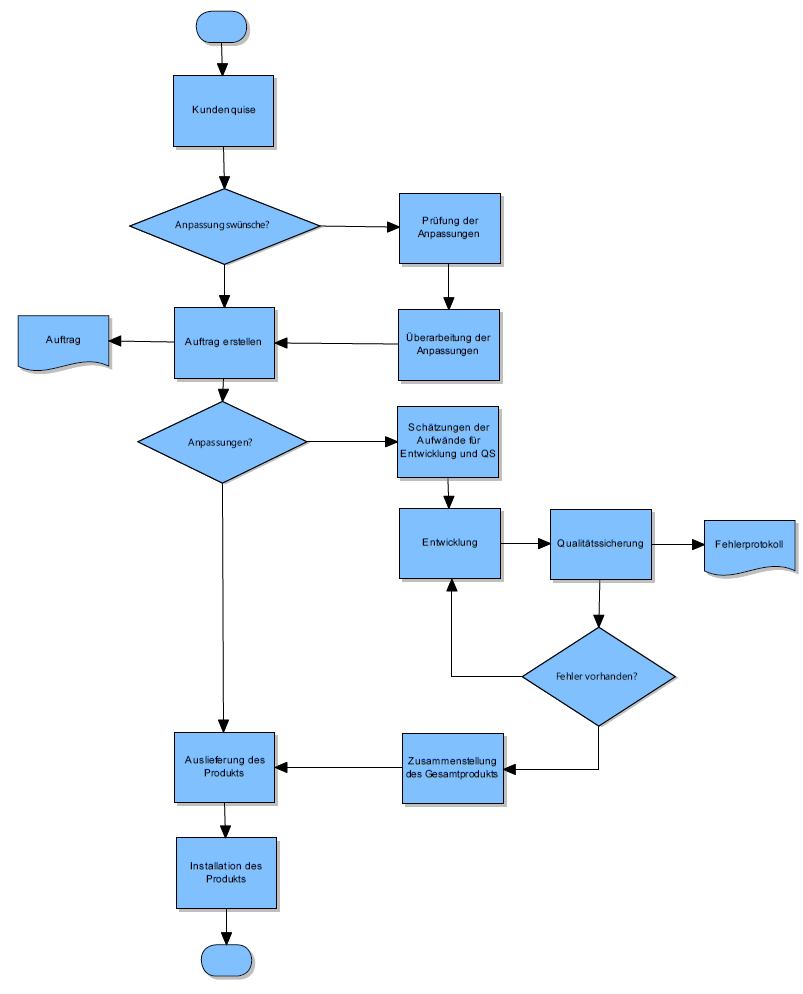
\includegraphics[width=0.9\textwidth]{Diagramm}
\caption{Flussdiagramm eines Projektablaufs}
Quelle: Eigene Darstellung
\end{center}
\end{figure}
\vspace{-1cm}

Diese Projektart bezieht sich auf die Akquisition von Neukunden. Auch Bestandskunden können neue Projekte in Auftrag geben, wobei hier wieder zwischen zwei verschiedenen Projektgegenständen unterschieden wird. Zum einen können zu den bereits erworbenen Modulen weitere hinzugekauft werden. Dabei besteht erneut die Möglichkeit, dass der Kunde verschieden Anpassungen wünscht, die es zu prüfen und zu realisieren gilt. Außerdem können selbst im laufenden Betrieb Anpassungswünsche auftreten, welche durch einen sogenannten CR (Change Request)\nomenclature{CR}{Change Request} beauftragt werden. Dieser wird durch den zuständigen Kundenberater des Unternehmens in Zusammenarbeit mit einem kundenseitigen Ansprechpartner erstellt. Der Projektablauf gleicht anschließend dem beim Ersterwerb.

\subsubsection{Teambildung}
Für ein Projekt werden keine expliziten Teams definiert. Vielmehr existieren pro Modul ein oder zwei Spezialisten, die besonderes Wissen dazu besitzen oder sogar maßgeblich an der initialen Entwicklung des entsprechenden Moduls beteiligt waren. Die Module bestehen dabei aus einzelnen Programmen, welche wiederrum einen unterschiedlichen Komplexitätsgrad aufweisen können. Daher kann es vorkommen, dass bestimmte Programme aufgrund ihrer Komplexität nur vom erfahrensten Entwickler bearbeitet werden können. Da die Entwickler aufgrund ihrer geringen Anzahl neben den Projektaufträgen auch das Tagesgeschäft erledigen müssen, werden sie nicht für die einzelnen Aufträge abgestellt. Sie müssen zeitweise bei Bedarf mehrere Aufträge gleichzeitig bearbeiten, gleiches gilt auch für die Mitarbeiter der Qualitätssicherung.

\subsubsection{Zuständigkeiten}
Welche Aufgaben von welchem Entwickler bzw. Tester übernommen werden, entscheidet zentral der Bereichsleiter. Er prüft die zu implementierende Anpassung, weist diese seinem Ermessen nach dem zuständigen Spezialisten zur Prüfung und schließlich zur Bearbeitung zu und bestimmt einen Tester. Dieser muss ebenfalls genügend Erfahrung mit dem Modul bzw. dem Programm besitzen, um sinnvolle Testfälle aufstellen zu können. Tritt kurzfristig ein dringliches Anliegen für ein Programm auf, dessen Spezialist bereits in einem Projekt tätig ist, muss dieser seine Arbeit unterbrechen und sich um das Anliegen kümmern. Der Tester ist zuständig für die Qualität des Programms. Er erstellt nach seinem Test ein Testprotokoll, in welchem die Testfälle und Fehler festgehalten werden, und stellt dieses für den Entwickler zur Korrektur bereit. Außerdem erstellt er die Dokumentation der getätigten Anpassung.

\subsubsection{Kommunikation}
Die einzelnen Entwickler, welche die verschiedenen Anpassungen eine Projekts realisieren, stimmen sich kaum untereinander ab. Treten Probleme oder Fragen auf, wird sich diesbezüglich kurz ausgetauscht. Nach Abschluss der Anpassung wendet sich unter Umständen der Tester an den Entwickler zur genaueren Erläuterung und Klärung von Verständnisfragen. Kommunikation zum Kunden besteht zunächst lediglich zu Beginn des Projekts. Hierbei stimmt der Projektleiter seitens des Unternehmens die gewünschten Anpassungen mit dem kundenseitigen Projektleiter ab. Zusätzlich kann ein Entwickler bei Fragen den Kunden selbstständig kontaktieren, es besteht somit keine geregelter Kommunikationsweg zum Kunden.

\subsection{SOLL-Analyse}
\subsubsection{Anforderungen}
Das neu einzuführende Prozessmodell soll bestimmte spezifizierte Anforderungen möglichst vollständig erfüllen können. Das Hauptaugenmerk liegt hierbei auf der optimierten Ressourcen- und Zeitausnutzung, da den Mitarbeitern aufgrund der Anzahl und Größe der Projekte mehrere Aufgaben parallel zugewiesen werden. Dies führt zu einer erhöhten Auslastung der Entwickler und Qualitätssicherer. Infolgedessen können Termingrenzen nicht immer eingehalten werden. Durch eine gezieltere Aufgabenteilung und Teambildung soll hier eine Optimierung erreicht werden, welche sowohl die Effizienz als auch die Entwicklungsdauer umfasst.\footcite[Vgl.][]{interview}

Das neue Prozessmodell soll die Bildung von abgegrenzten Projektteams vorsehen und gleichzeitig eine geringe Anzahl an Mitarbeitern pro Team favorisieren. Der Grund hierfür ist die geringe Anzahl an verfügbaren Entwicklern in Verbindung mit der parallelen Bearbeitung mehrerer Projekte. Zusätzlich sollen neue und unerfahrene Mitarbeiter an die Programme herangeführt werden und möglichst umfangreiche Kenntnisse in unterschiedlichen Fachgebieten erlangen, um das Wissen im Unternehmen maximal zu streuen. Dadurch soll der Schaffung von Spezialisten für die einzelnen Programme und Module entgegengewirkt werden.\footcite[Vgl.][]{interview}

Um zeitliche Engpässe während der gesamten Projektarbeit zu umgehen, soll im Allgemeinen durch Prozessoptimierungen und -vereinheitlichungen in den einzelnen Bereichen eine Verkürzung der gesamten Durchlaufzeit erreicht werden. Ebenfalls soll ein kundenseitiger Ansprechpartner enger in die Entwicklung eingebunden werden. Aufgrund notwendiger Abstimmungen während der Realisierungsphase soll sowohl ein einheitlicher und direkter Kommunikationsweg zum Kunden geschaffen, als auch die Frequenz derselben erhöht werden. Dies soll bezüglich der Spezifikationen auftretende Probleme simpler und schneller lösbar machen. Des Weiteren muss die Kundenanpassung zwingend in Form einer Anwenderdokumentation zur Unterstützung des Endbenutzers und zur Aufwandsminimierung bei der Entwicklung weiterer Anpassung festgehalten werden.\footcite[Vgl.][]{interview}

\subsubsection{Wünsche}
Zum einen besteht der Wunsch, dass das gesamte Wissen bezüglich Entwicklung und Qualitätssicherung nicht auf einzelne Spezialisten verteilt ist, sondern jeder Entwickler und Tester jede Art von Projekt übernehmen können. Besonders Entwickler müssen in der Lage sein, Anpassungen für jedes Programm prüfen, schätzen und implementieren zu können, unabhängig vom Komplexitätsgrad. Zusätzlich wäre die Realisierung eines integrierten Risikomanagements wünschenswert. Es sollen Risiken analysiert, geprüft und verhindert bzw. minimiert werden können, da diesbezüglich zurzeit keinerlei Aktivitäten im Unternehmen stattfinden. Dadurch sollen plötzlich auftretende Notsituationen wie Krankheitsfälle entschärft werden können.\footcite[Vgl.][]{interview}